\documentclass[../../main.tex]{subfiles}
\begin{document}
\begin{oframed}
  \subfile{problem}
\end{oframed}

{\bf [解答]} $g(x)=f(x)-ax$とおく．
\begin{align}
  g(x)=
  \begin{cases}
    -ax+1&(1\le x\le 2) \\
    (1-a)x-1&(2\le x\le3)
  \end{cases}
\end{align}
である($g(x)$は連続)．$a$の値によって以下のようになる．

\noindent\underline{(i)$a\le0$の時}

$g(x)$は増加関数だから，
\begin{align}
  V(a)=g(3)-g(1)=1-2a
\end{align}

\noindent\underline{(ii)$0\le a\le 1$の時}

$g(x)$のグラフの概形は下図．

\begin{figure}[htb]
  \centering
  % 左パネル: 0 <= a <= 1 における g(x) のグラフ
  \begin{subcaptionblock}{0.48\textwidth}
    \centering
    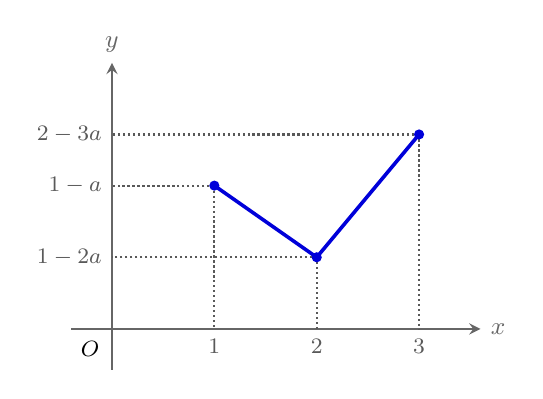
\begin{tikzpicture}[x=1.3cm, y=1.3cm, >=stealth, every node/.style={font=\small}]
      % 座標軸
      \draw[->, thick, gray!80!black] (-0.4, 0) -- (3.6, 0) node[right] {$x$};
      \draw[->, thick, gray!80!black] (0, -0.4) -- (0, 2.6) node[above] {$y$};
      \node[below left=1pt, font=\footnotesize] at (0, 0) {$O$};

      % 折れ線: a = 1/4 を例とする (1-a = 0.75, 1-2a = 0.5, 2-3a = 1.25 をスケール調整)
      \coordinate (A) at (1, 1.4);
      \coordinate (B) at (2, 0.7);
      \coordinate (C) at (3, 1.9);

      \draw[line width=1.3pt, blue!85!black] (A) -- (B) -- (C);

      % 垂線 (x軸, y軸)
      \draw[densely dotted, thick, gray!70!black] (A) -- (1, 0) node[below, font=\footnotesize] {$1$};
      \draw[densely dotted, thick, gray!70!black] (B) -- (2, 0) node[below, font=\footnotesize] {$2$};
      \draw[densely dotted, thick, gray!70!black] (C) -- (3, 0) node[below, font=\footnotesize] {$3$};

      \draw[densely dotted, thick, gray!70!black] (A) -- (0, 1.4) node[left, font=\footnotesize] {$1-a$};
      \draw[densely dotted, thick, gray!70!black] (B) -- (0, 0.7) node[left, font=\footnotesize] {$1-2a$};
      \draw[densely dotted, thick, gray!70!black] (C) -- (0, 1.9) node[left, font=\footnotesize] {$2-3a$};

      % 代表点
      \node[circle, fill=blue!85!black, inner sep=1.3pt] at (A) {};
      \node[circle, fill=blue!85!black, inner sep=1.3pt] at (B) {};
      \node[circle, fill=blue!85!black, inner sep=1.3pt] at (C) {};
    \end{tikzpicture}
    \caption{$0 \le a \le 1$ における $g(x)$ の概形}
    \label{fig:gx_graph}
  \end{subcaptionblock}
  \hfill
  % 右パネル: V(a) のグラフ
  \begin{subcaptionblock}{0.48\textwidth}
    \centering
    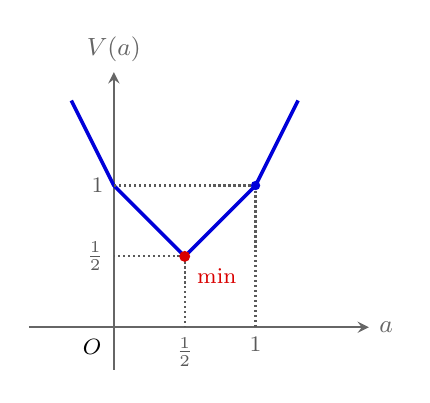
\begin{tikzpicture}[x=1.8cm, y=1.8cm, >=stealth, every node/.style={font=\small}]
      % 座標軸
      \draw[->, thick, gray!80!black] (-0.6, 0) -- (1.8, 0) node[right] {$a$};
      \draw[->, thick, gray!80!black] (0, -0.3) -- (0, 1.8) node[above] {$V(a)$};
      \node[below left=1pt, font=\footnotesize] at (0, 0) {$O$};

      % 折れ線: (-0.3, 1.6) -> (0, 1) -> (0.5, 0.5) -> (1, 1) -> (1.3, 1.6)
      \draw[line width=1.3pt, blue!85!black]
      (-0.3, 1.6) -- (0, 1.0) -- (0.5, 0.5) -- (1.0, 1.0) -- (1.3, 1.6);

      % 最小点 (0.5, 0.5)
      \coordinate (M) at (0.5, 0.5);
      \coordinate (P1) at (1.0, 1.0);

      \draw[densely dotted, thick, gray!70!black] (M) -- (0.5, 0) node[below, font=\footnotesize] {$\frac{1}{2}$};
      \draw[densely dotted, thick, gray!70!black] (M) -- (0, 0.5) node[left, font=\footnotesize] {$\frac{1}{2}$};

      \draw[densely dotted, thick, gray!70!black] (P1) -- (1.0, 0) node[below, font=\footnotesize] {$1$};
      \draw[densely dotted, thick, gray!70!black] (P1) -- (0, 1.0) node[left, font=\footnotesize] {$1$};

      \node[circle, fill=red!85!black, inner sep=1.4pt] at (M) {};
      \node[below right=1pt, font=\footnotesize, text=red!85!black] at (M) {$\min$};
      \node[circle, fill=blue!85!black, inner sep=1.2pt] at (P1) {};
    \end{tikzpicture}
    \caption{$V(a)$ のグラフ}
    \label{fig:va_graph}
  \end{subcaptionblock}
  \caption{$g(x)$ の概形と $V(a)$ の挙動}
  \label{fig:1973_3_graphs}
\end{figure}

また
\begin{align}
  \begin{cases}
    g(3)\ge g(1)&(0\le a\le 1/2) \\
    g(3)\le g(1) &(1/2\le a\le 1)
  \end{cases}
\end{align}
であるから，
\begin{align}
  V(a)=&
  \begin{cases}
    g(3)-g(2)&(0\le a\le 1/2)\\
    g(1)-g(2)&(1/2\le a\le 1)
  \end{cases} \\
  =&
  \begin{cases}
    1-a&(0\le a\le 1/2)\\
    a&(1/2\le a\le 1)
  \end{cases}
\end{align}

\noindent\underline{(iii)$1\le a$の時}

$g(x)$は減少関数だから，
\begin{align}
  V(a)=g(1)-g(3)=2a-1
\end{align}

以上から，$\min V(a)=V(1/2)=1/2$である．$\cdots$(答)

\newpage
\end{document}
